\section{Results}
\label{sec:results}

In this section, we demonstrate the use of LOBE to block-encode Hamiltonians, and compare these results with the cost associated with block encoding these Hamiltonians with a standard LCU approach.
To compare with LCU, each Hamiltonian will be transformed to Paulis with the Jordan-Wigner \cite{jordan-wigner} and standard binary \cite{standard-binary} for fermions and bosons respectively. \gus{@Will, do we need to add the SB mapping to the appendix?}
There are four Hamiltonians we show results for: two non-relativistic Hamiltonians (static massive Yukawa, and quartic harmonic oscillator), and two fully relativistic quantum field theory models (full massive Yukawa, and $\phi^4$ theory).
The costs associated with a block encoding are determined by looking at numerical counts for the numbers of non-Clifford operations, the number of ancillae required beyond the system register, and the rescaling factor imposed on the resulting block-encoding.

The results that we present here are generated based on constructions of LOBE that are written in Cirq \cite{cirq} and the block-encodings are numerically verified for circuits of up to 14 qubits.
Additionally, the operators are constructed through the use of OpenParticle \cite{openparticle}, a software library for the construction and manipulation of fermionic, antifermionic, and bosonic ladder operators.
The software library \cite{grover-rudolph-github} is used to determine the rotation angles required for Grover-Rudolph.

The first two models below can be thought of as corresponding to a full quantum field theory constrained to a single mode, reducing it to a quantum mechanics problem.

% In this section, we demonstrate the use of LOBE to block-encode Hamiltonians derived from quantum field theories: Yukawa theory and $\phi^4$ theory \cite{Peskin:1995ev}.
% We study both variants of the block-encoding described in Sections \ref{sec:block-encoding} and expanded upon in Section \ref{sec:lobe} and give numerical counts for the numbers of non-Clifford operations, the number of ancillae required beyond the system register, and the rescaling factor imposed on the resulting block-encoding.

% The results that we present here are generated based on constructions of LOBE that are written in Cirq \cite{cirq} and the block-encodings are numerically verified for circuits of up to 14 qubits.
% Additionally, the operators are constructed through the use of OpenParticle \cite{openparticle}, a software library for the construction and manipulation of fermionic, antifermionic, and bosonic ladder operators.
% The software library \cite{grover-rudolph-github} is used to determine the rotation angles required for Grover-Rudolph.

% \subsection{Yukawa Theory}
% A quantum field theory that models the strong nuclear force between hadrons is Yukawa theory \cite{Peskin:1995ev}. In this theory, hadrons are described by a fermionic field $\psi$, coupled via a scalar boson $\phi$. The interaction term is $\mathcal{L}_{\text{Yukawa}} = g\bar\psi \psi \phi$, which leads to interaction vertices containing fermions and/or antifermions and bosons. The Lagrangian, and thus the Hamiltonian, is written as a sum of free, non-ineteracting fields and the interaction term.

% Utilizing the lightfront frame \cite{Dirac1949}, leads to a straightforward approach to writing down the Hamiltonian bound-state eigenvalue equation in terms of ladder operators. This lightfront frame removes the ambiguous $\sqrt{\nabla^2 + m^2}$ term that appears in a canonical, instant-time frame Hamiltonian approach. 

% The interaction terms in the Hamiltonian are $H_{\text{Yukawa int}} \in \{b^\dagger b a, b^\dagger b a^\dagger, d^\dagger d a, d^\dagger d a^\dagger, b^\dagger d^\dagger a, bda^\dagger, b^\dagger b a^\dagger a, d^\dagger d a^\dagger a \}$, while the free part of the Hamiltonian is $H_{\text{free}} \in \{b^\dagger b, d^\dagger d, a^\dagger a \}$. 
% Much of the interesting physics arises from the interacting piece. The terms $b^\dagger b a$ and $b^\dagger b a^\dagger$ describe the annihilation of a fermion with a boson and creation of a fermion, and the creation of a fermion-boson pair from a fermion respectively. $d^\dagger d a$ and $d^\dagger d a^\dagger$ describe the same interactions but for antifermions and bosons. 
% $b^\dagger d^\dagger a$ and $bda^\dagger$ correspond to fermion-antifermion pair creation and annihilation, and lastly, $b^\dagger b a^\dagger a$ and $d^\dagger d a^\dagger a$ are terms of $\mathcal{O}(g^2)$, unique to the lighfront frame.

% This Hamiltonian can be written out as a discrete sum over these free and interaction ladder operators with coefficients coming from lightfront coordinates. The Hamiltonian can be written as:

% \begin{equation}
%     \label{eq:Yukawa-hamiltonian}
%     H_{\text{Yukawa}} = H_0 + H_{\bar\psi \psi \phi}.
% \end{equation}
% The explicit form of the Hamiltonian will be written out in the appendix \ref{subsec:lightfront-hamiltonian}.

% \begin{figure}
%     \centering
%     \includegraphics[width=16cm]{figures/Yukawa_hamiltonian_gates_vs_terms.pdf}
%     \caption{
%         \textbf{Numerical Gate Counts for Increasing $L$ (Yukawa Hamiltonian).}
%         The number of rotations (left), left-elbows (middle), and right-elbows (right) are plotted as a function of the number of terms in the Hamiltonian ($L$) for an increasing number of momentum modes ($I$).
%         The gate counts for the variant of LOBE using \textit{USP} are shown as the blue squares.
%         The gate counts for the variant of LOBE using \textit{ASP} are shown as the orange circles.
%         The bosonic occupancy cutoff ($\Omega$) is set to $3$.
%         The number of rotations excludes rotations by angles that result in Clifford operations.
%     }
%     \label{fig:Yukawa_hamiltonian_gates_vs_terms}
% \end{figure}
% \begin{figure}
%     \centering
%     \includegraphics[width=12cm]{figures/Yukawa_hamiltonian_qubits_and_rescaling_vs_terms.pdf}
%     \caption{
%         \textbf{Numerical Ancillae Counts and Rescaling Factors for Increasing $L$ (Yukawa Hamiltonian).}
%         The number of required ancillae (left) and the resulting rescaling factor (right) for LOBE are plotted as a function of the number of terms in the Hamiltonian ($L$) for an increasing number of momentum modes ($I$).
%         The counts for the variant of LOBE using \textit{USP} are shown as the blue squares.
%         The counts for the variant of LOBE using \textit{ASP} are shown as the orange circles.
%         The bosonic occupancy cutoff ($\Omega$) is set to $3$.
%     }
%     \label{fig:Yukawa_hamiltonian_qubits_and_rescaling_vs_terms}
% \end{figure}

% In Figure \ref{fig:Yukawa_hamiltonian_gates_vs_terms}, we plot the numerical gate counts estimates for the Yukawa Hamiltonian (Eq. \ref{eq:Yukawa-hamiltonian}) as the number of terms in the Hamiltonain ($L$) increases.
% The number of terms ($L$) increases directly with an increasing number of momentum modes as $\mathcal{O}(I^3)$.
% For the three non-Clifford operations, the number of operations increases linearly with the number of terms in the Hamiltonian for this model.
% Additionally, the two different compilation strategies (\textit{USP} (blue), \textit{ASP} (orange)) demonstrate the same numerical scaling and have nearly identical gate counts for all types of operations.
% When the number of terms ($L$) is far from the next largest power of 2, \textit{ASP} requires more arbitrary rotations due to the compilation of Grover-Rudolph and multiplexed rotations that is used in this work.

% In Figure \ref{fig:Yukawa_hamiltonian_qubits_and_rescaling_vs_terms}, we plot the numerical estimates for the number of required ancillae (left) and the imposed rescaling factor (right) as the number of terms in the Hamiltonain ($L$) increases.
% The number of ancillae grows logarithmically with the number of terms for both implementations.
% The number of ancillae used for the index register grows logarithmically with the number of terms which accounts for this scaling.
% The main advantage of the \textit{ASP} variant is the effect on the rescaling factor of the block-encoding.
% While the rescaling factor of both variants seemingly grows linearly with respect to the number of terms in the Hamiltonian, the rescaling factor for the \textit{ASP} variant is significantly smaller than the \textit{USP} variant.
% When block-encodings are employed as a subroutine in larger algorithms, the quantum resources for the algorithm are often dependent on the rescaling factor (with a lower rescaling factor generally being preferred).
% For example, in the context of using Quantum Phase Estimation to estimate the eigenvalues of a Hamiltonian, the number of gates required typically scales as $O(\frac{1}{\lambda})$ \cite{babbush2018encoding}. 
% However, the exact cost associated with the rescaling factor is difficult to determine without choosing a specific algorithm to benchmark with.

% \begin{figure}
%     \centering
%     \includegraphics[width=16cm]{figures/Yukawa_hamiltonian_gates_vs_omega.pdf}
%     \caption{
%         \textbf{Numerical Gate Counts for Increasing $\Omega$ (Yukawa Hamiltonian) .}
%         The number of rotations (left), left-elbows (middle), and right-elbows (right) are plotted as a function of the bosonic occupation cutoff ($\Omega$).
%         The gate counts for the variant of LOBE using \textit{USP} are shown as the blue squares.
%         The gate counts for the variant of LOBE using \textit{ASP} are shown as the orange circles.
%         The number of momentum modes ($I$) is set to $2$.
%         The number of rotations excludes rotations by angles that result in Clifford operations.
%     }
%     \label{fig:Yukawa_hamiltonian_gates_vs_omega}
% \end{figure}
% \begin{figure}
%     \centering
%     \includegraphics[width=12cm]{figures/Yukawa_hamiltonian_qubits_and_rescaling_vs_omega.pdf}
%     \caption{
%         \textbf{Numerical Ancillae Counts and Rescaling Factors for Increasing $\Omega$ (Yukawa Hamiltonian).}
%         The number of required ancillae (left) and the resulting rescaling factor (right) for LOBE are plotted as a function of the bosonic occupation cutoff ($\Omega$).
%         The counts for the variant of LOBE using \textit{USP} are shown as the blue squares.
%         The counts for the variant of LOBE using \textit{ASP} are shown as the orange circles.
%         The number of momentum modes ($I$) is set to $2$.
%     }
%     \label{fig:Yukawa_hamiltonian_qubits_and_rescaling_vs_omega}
% \end{figure}

% In Figure \ref{fig:Yukawa_hamiltonian_gates_vs_omega}, we plot the numerical gate counts estimates for the Yukawa Hamiltonian (Eq. \ref{eq:Yukawa-hamiltonian}) as the cutoff on the maximum bosonic occupation ($\Omega$) increases.
% For the three non-Clifford operations, the number of operations increases linearly with the bosonic occupancy cutoff for this model.
% Similar to the case with increasing $I$, the two different compilation strategies (\textit{USP} (blue), \textit{ASP} orange) demonstrate the same numerical scaling and have nearly identical gate counts for all types of operations.

% In Figure \ref{fig:Yukawa_hamiltonian_qubits_and_rescaling_vs_omega}, we plot the numerical estimates for the number of required ancillae (left) and the imposed rescaling factor (right) as the cutoff on the maximum bosonic occupation ($\Omega$) increases.
% The number of ancillae grows logarithmically with the bosonic occupation cutoff for both implementations.
% The number of ancillae needed to update the bosonic occupancy grows logarithmically with $\Omega$ (Eq. \ref{eq:ancillae-bosonic-updates}) which accounts for this scaling.
% Again, the main advantage of the \textit{ASP} variant is that the imposed rescaling factor is significantly smaller than the \textit{USP} variant, especially for large values of $\Omega$ despite the asymptotic scaling being linear for both.

% It is important to note about the rescaling factor ($\lambda$) with the occupation cutoff ($\Omega$). For both \textit{USP} and \textit{ASP}, the rescaling factors depend on $\lambda_A$ \ref{eq:bosonic-rescaling-factor}, which is proportional to $\Omega^{A/2}$. 
% For Yukawa theory, $A$, is fixed to 2 (this comes from the free piece $\sim a^\dagger a$). Thus, $(\Omega + 1)^{A/2}$ gives linear scaling. 


% \subsection{$\phi^4$ Theory}
% Another interesting field theoretical application of LOBE comes from a purely bosonic theory: $\phi^4$. This model describes a self-interacting bosonic field with $\mathcal{L}_{int} = g\phi^4$. 
% There are three main interaction first order vertices in this theory: 2 bosons $\rightarrow$ 2 bosons: $a^\dagger a^\dagger a a$, 1 boson $\rightarrow$ 3 bosons: $a^\dagger a^\dagger a^\dagger a$, and 3 bosons $\rightarrow$ 1 boson: $a^\dagger a a a$. 
% The explicit form of the Hamiltonian is given in appendix \ref{subsec:lightfront-hamiltonian}.

% Figures \ref{fig:phi4_hamiltonian_gates_vs_terms} and \ref{fig:phi4_hamiltonian_qubits_and_rescaling_vs_terms} show the scaling of gates and qubits needed to simulate the $\phi^4$ Hamiltonian with LOBE as the number of terms in the Hamiltonian ($L$) increases. 
% In the same way as the Yukawa Hamiltonian, the number of terms ($L$) increases directly with an increasing number of momentum modes as $\mathcal{O}(I^3)$. The scaling for the two different compilation strategies (\textit{USP} (blue), \textit{ASP} (orange)) demonstrate the same numerical scaling and have nearly identical gate counts for all types of operations. 

% Figures \ref{fig:phi4_hamiltonian_gates_vs_omega} and \ref{fig:phi4_hamiltonian_qubits_and_rescaling_vs_omega} show the scaling of gates and qubits needed to simulate the $\phi^4$ Hamiltonian with LOBE as the maximum bosonic occupancy ($\Omega$) increases. Similar to the case with increasing \textit{I}, the scaling for the two different compilation strategies (\textit{USP} (blue), \textit{ASP} (orange)) demonstrate the same numerical scaling and have nearly identical gate counts for all types of operations. 

% Again, the scaling of $\lambda$ with $\Omega$ must be mentioned. For $\phi^4$-theory, $A = 4$, (this comes from the interaction piece), so the scaling of $\lambda$ is $\sim \Omega^2$, which gives quadratic scaling for both \textit{USP} and \textit{ASP}.


% \begin{figure}
%     \centering
%     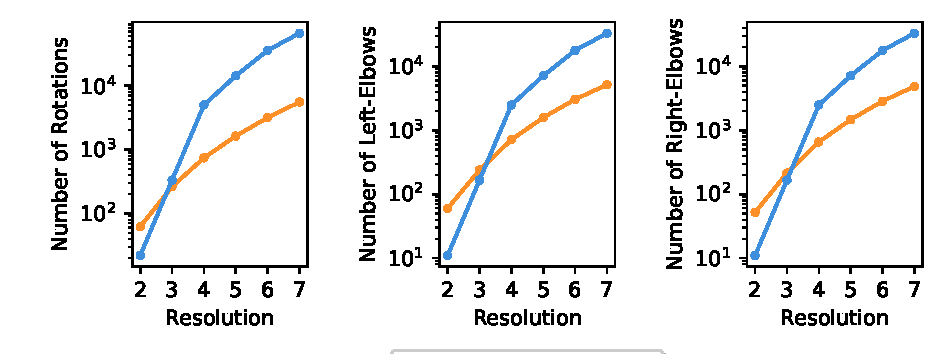
\includegraphics[width=16cm]{figures/phi4_hamiltonian_gates_vs_terms.pdf}
%     \caption{
%         \textbf{Numerical Gate Counts for Increasing $L$ ($\phi^4$ Hamiltonian).}
%         The number of rotations (left), left-elbows (middle), and right-elbows (right) are plotted as a function of the number of terms in the Hamiltonian ($L$) for an increasing number of momentum modes ($I$).
%         The gate counts for the variant of LOBE using \textit{USP} are shown as the blue squares.
%         The gate counts for the variant of LOBE using \textit{ASP} are shown as the orange circles.
%         The bosonic occupancy cutoff ($\Omega$) is set to $3$.
%         The number of rotations excludes rotations by angles that result in Clifford operations.
%     }
%     \label{fig:phi4_hamiltonian_gates_vs_terms}
% \end{figure}
% \begin{figure}
%     \centering
%     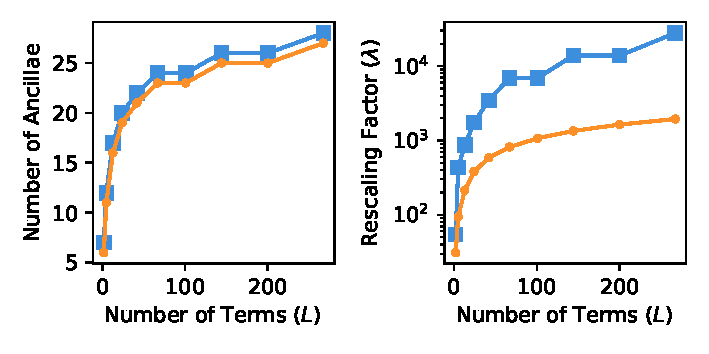
\includegraphics[width=12cm]{figures/phi4_hamiltonian_qubits_and_rescaling_vs_terms.pdf}
%     \caption{
%         \textbf{Numerical Ancillae Counts and Rescaling Factors for Increasing $L$ ($\phi^4$ Hamiltonian).}
%         The number of required ancillae (left) and the resulting rescaling factor (right) for LOBE are plotted as a function of the number of terms in the Hamiltonian ($L$) for an increasing number of momentum modes ($I$).
%         The counts for the variant of LOBE using \textit{USP} are shown as the blue squares.
%         The counts for the variant of LOBE using \textit{ASP} are shown as the orange circles.
%         The bosonic occupancy cutoff ($\Omega$) is set to $3$.
%     }
%     \label{fig:phi4_hamiltonian_qubits_and_rescaling_vs_terms}
% \end{figure}

% \begin{figure}
%     \centering
%     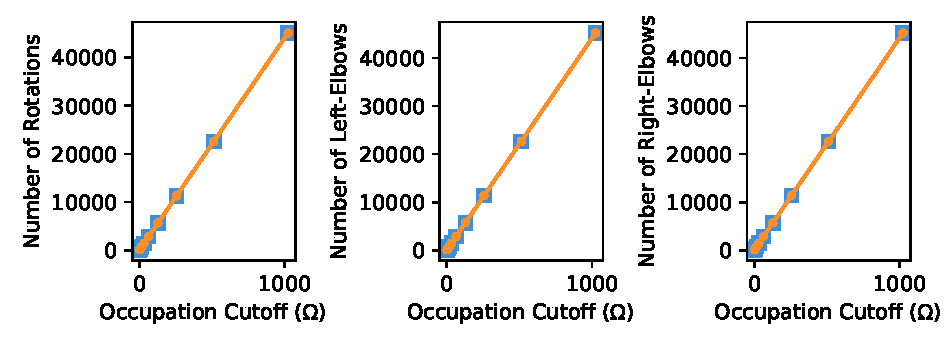
\includegraphics[width=16cm]{figures/phi4_hamiltonian_gates_vs_omega.pdf}
%     \caption{
%         \textbf{Numerical Gate Counts for Increasing $\Omega$ ($\phi^4$ Hamiltonian) .}
%         The number of rotations (left), left-elbows (middle), and right-elbows (right) are plotted as a function of the bosonic occupation cutoff ($\Omega$).
%         The gate counts for the variant of LOBE using \textit{USP} are shown as the blue squares.
%         The gate counts for the variant of LOBE using \textit{ASP} are shown as the orange circles.
%         The number of momentum modes ($I$) is set to $3$.
%         The number of rotations excludes rotations by angles that result in Clifford operations.
%     }
%     \label{fig:phi4_hamiltonian_gates_vs_omega}
% \end{figure}
% \begin{figure}
%     \centering
%     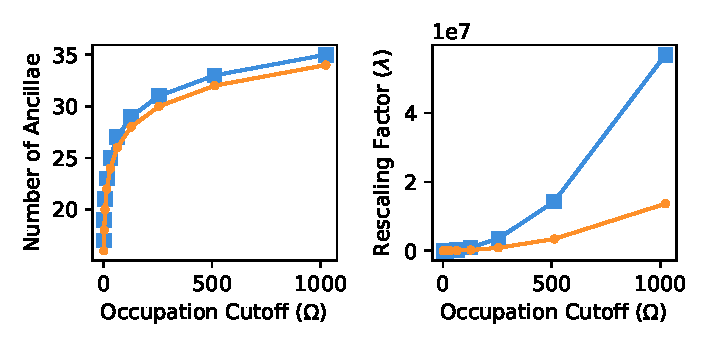
\includegraphics[width=12cm]{figures/phi4_hamiltonian_qubits_and_rescaling_vs_omega.pdf}
%     \caption{
%         \textbf{Numerical Ancillae Counts and Rescaling Factors for Increasing $\Omega$ ($\phi^4$ Hamiltonian).}
%         The number of required ancillae (left) and the resulting rescaling factor (right) for LOBE are plotted as a function of the bosonic occupation cutoff ($\Omega$).
%         The counts for the variant of LOBE using \textit{USP} are shown as the blue squares.
%         The counts for the variant of LOBE using \textit{ASP} are shown as the orange circles.
%         The number of momentum modes ($I$) is set to $3$.
%     }
%     \label{fig:phi4_hamiltonian_qubits_and_rescaling_vs_omega}
% \end{figure}